% Drawing 73/01-2 -- folder 73, batch 01, archive page 6 (PDF page 7).
% Transcription: sous le texte, cinq croquis de quadrilatères : un quadrilatère ouvert, un quadrilatère croisé en « Z », deux droites sécantes portant quatre points, un trapèze avec ses diagonales, un quadrilatère aplati avec ses diagonales
% Kind: sketches of quadrilaterals. Method 2 (schematic redraw from the facsimile). Status: ok.
% Notes: Five pencil sketches, left to right and top to bottom: an open quadrilateral (three sides, a tick at the free end); a crossed quadrilateral in Z; lines through four points, two of them thickened; a trapezoid with its two diagonals and a vertical stroke from a dot on the top side; a flattened quadrilateral with its diagonals (bottom left, with a faint stroke under it). Disagreement (minor): the "deux droites sécantes" sketch shows three lines (two long lines and a third through two of the points), with two short thick strokes between the points.
% Coordinates: 1 unit = 1 mm = 1/100 of the crop width (bbox in page fractions: [0.08, 0.37, 0.8, 0.52]).
% Redrawn by Claude (claude-opus-5-5), issue #73, 2026-11-07; not checked by a human; not compiled (no TeX in the session).
% Rights: reproduces part of the work -- behind RENDER_TRANSCRIPTS, never published by itself.
\documentclass[tikz,border=3pt]{standalone}
\usepackage{amsmath,amssymb}
\usetikzlibrary{patterns,arrows.meta}
\tikzset{pencil/.style={black!45}, struck/.style={black!35}, mark/.style={circle,draw,inner sep=1.3pt}, pt/.style={circle,fill,inner sep=0.9pt}, opt/.style={circle,draw,fill=white,inner sep=1.1pt}}
\begin{document}
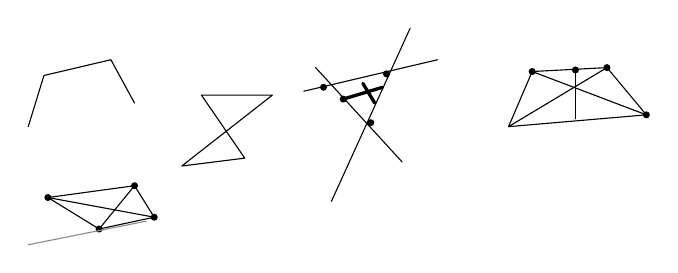
\begin{tikzpicture}[x=1mm,y=1mm,line cap=round,line join=round,font=\scriptsize]
\draw (8,-13.5) -- (10,-7) -- (18.5,-5) -- (21.5,-10.5);
\draw (30,-9.5) -- (39,-9.5) -- (27.5,-18.5) -- (35.5,-17.5) -- cycle;
\draw (43,-9) -- (60,-5);
\draw (56.5,-1) -- (46.5,-23);
\draw (44.5,-6) -- (55.5,-18);
\draw[very thick] (48,-10) -- (53,-8.5);
\draw[very thick] (50.5,-8) -- (52,-10.5);
\node[pt] at (45.5,-8.5) {};
\node[pt] at (53.5,-6.8) {};
\node[pt] at (51.5,-13) {};
\node[pt] at (48,-10) {};
\draw (72,-6.5) -- (81.5,-6) -- (86.5,-12) -- (69,-13.5) -- cycle;
\draw (72,-6.5) -- (86.5,-12);
\draw (81.5,-6) -- (69,-13.5);
\draw (77.5,-6.3) -- (77.5,-12.5);
\node[pt] at (72,-6.5) {};
\node[pt] at (81.5,-6) {};
\node[pt] at (86.5,-12) {};
\node[pt] at (77.5,-6.3) {};
\draw (10.5,-22.5) -- (21.5,-21) -- (24,-25) -- (17,-26.5) -- cycle;
\draw (10.5,-22.5) -- (24,-25);
\draw (21.5,-21) -- (17,-26.5);
\node[pt] at (10.5,-22.5) {};
\node[pt] at (21.5,-21) {};
\node[pt] at (24,-25) {};
\node[pt] at (17,-26.5) {};
\draw[pencil] (8,-28.5) -- (23,-25.5);
\end{tikzpicture}
\end{document}
